\documentclass[12pt,a4paper,utf8x]{article}
\usepackage{lmodern}
\usepackage[T1]{fontenc} 
\usepackage[utf8]{inputenc}  
\usepackage [frenchb]{babel}

% Pour pouvoir utiliser le verbatim dans les sections utiliser la commande versalitas
\newcommand{\versalitas}[1]{{\usefont{T1}{cmr}{bx}{sc}#1}}% 

\usepackage{textcomp}
\usepackage{keystroke}
\usepackage{amssymb}
 
\usepackage{amsmath}
\renewcommand{\thesection}{\arabic{section}} % numérotation des sectiosn
\usepackage[cc]{titlepic} %rajouter le logo dans la page de garde
\usepackage{url} % Pour avoir de belles url
\usepackage {geometry}
\usepackage[linktocpage]{hyperref}

%enlever le numéro de page
\usepackage{nopageno}
% Pour mettre du code source
\usepackage {listings}
% Pour pouvoir passer en paysage
\usepackage{lscape}	

% Pour pouvoir faire plusieurs colonnes
\usepackage {multicol}

% POur crééer un index
\usepackage{makeidx}

\usepackage[pdftex]{graphicx}

\hypersetup{
backref=true,
%permet d'ajouter des liens dans...
pagebackref=true,%...les bibliographies
hyperindex=true, %ajoute des liens dans les index.
colorlinks=true, %colorise les liens
breaklinks=true, %permet le retour à la ligne dans les liens trop longs
urlcolor= blue, %couleur des hyperliens
citecolor=	cyan,
bookmarks=true, %créé des signets pour Acrobat
bookmarksopen=true,
%si les signets Acrobat sont créés,
%les afficher complètement.
pdftitle={Initiation à la Recherche}, %informations apparaissant dans
pdfauthor={MARGUERITE Alain\\ RINCE Romain},
%dans les informations du document
pdfsubject={Doc}
%sous Acrobat.
}
\hyphenation{si-tu-a-tion}
\makeindex


%%%% debut macro pour enlever le nom chapitre %%%%
% \makeatletter
% \def\@makechapterhead#1{%
%   \vspace*{50\p@}%
%   {\parindent \z@ \raggedright \normalfont
%     \interlinepenalty\@M
%     \ifnum \c@secnumdepth >\m@ne
%         \Huge\bfseries \thechapter\quad
%     \fi
%     \Huge \bfseries #1\par\nobreak
%     \vskip 40\p@
%   }}
% 
% \def\@makeschapterhead#1{%
%   \vspace*{50\p@}%
%   {\parindent \z@ \raggedright
%     \normalfont
%     \interlinepenalty\@M
%     \Huge \bfseries  #1\par\nobreak
%     \vskip 40\p@
%   }}
% \makeatother
%%%% fin macro %%%%

%Couverture 

%Couverture 
\widowpenalty=10000
\clubpenalty=10000
 
 \title{{\large \textbf{Résumé d'article}\\\emph{Applying Event and Machine Decomposition to a Flash-Based Filestore in Event-B}\\\vspace{0.2cm}
 {\scriptsize K. \textsc{Damchoom} and M. \textsc{Butler}\\\vspace{-0.5cm}University of Southampton}}}
%\titlepic{
\includegraphics[scale=0.80]{img/logouniv}}
		

\author{\small Romain \textsc{Rincé}\\{\small Encadrant : Christian \textsc{Attiogbé}}}
\date{}
 
%\title{{\Huge Formal Software Engineering}\\{\small Encadrant : Christian \textsc{Attiogbé}}\\\vspace{3cm} Résumé d'article :\\\vspace{0.3cm}{\Large \emph{Applying Event and Machine Decomposition to a Flash-Based Filestore in Event-B}}\\\vspace{0.3cm}
%\small K. \textsc{Damchoom} and M. \textsc{Butler}\\University of Southampton\\\vspace{2cm}}
%\titlepic{
\includegraphics[scale=0.80]{img/logouniv}}
		

%\author{\vspace{2cm}Romain \textsc{Rincé}}
%\date{\small Université de Nantes \\ 2 rue de la Houssinière, BP92208, F-44322 \textsc{Nantes} cedex 03, \textsc{France}}

\hyphenation{appar-tiennent}
\hyphenation{pro-blèmes}

\begin{document}

\maketitle
\renewcommand{\labelitemi}{$\bullet$} 


\section{Contexte}
Le papier \emph{Applying Event and Machine Decomposition to a Flash-Based Filestore in Event-B} présente un moyen de réprésenter, grâce à la méthode formelle~\emph{Event-B}, un système de fichier géré dans une mémoire flash. L'étude effectuée repose sur un autre travail précédemment effectué par les auteurs dans lequel ils explicitent un modèle abstrait d'un système arborescent de fichiers.

Le papier présente donc les différentes méthodes employées pour parvenir au modèle flash, tel que le raffinement et la décomposition de machine.

\section{Problématique}
La difficulté étant de réussir à faire coïncider un modèle formel avec un système de fichier ayant des contraintes physiques fortes et de s'assurer de la validité des opérations effectuées sur le support ; en particuler les opérations d'écriture qui sont relativement sensibles à l'erreur. Les auteurs prennent donc en compte, dans leur modélisation, les possibles erreurs d'écriture du support flash.

\section{Résultats}
Les auteurs obtiennent, au final, un modèle viable qu'ils prouvent par la suite grâce à \emph{Rodin}. Le modèle présenté sépare la partie \og système de fichier\fg{} de la partie \og interface flash\fg{} qui assure une certaine lisibilité et un meilleure taux de preuve automatique. Les auteurs mettent en effet en évidence que $93 \%$ des obligations de preuve sont effectué par \emph{Rodin} de manière automatique.

Certains problèmes restent tout de même en suspens, notamment le traitement de l'obscolescence du support flash ainsi que la technique de \emph{wear-levelling}\footnote{Il s'agit d'une technique permettant de prolonger la durée de vie de la mémoire flash} qui en découle. Du point de vue de Rodin, les auteurs indiquent que le logiciel ré-effectue, après une modification du modèle, certaines preuves qui ne sont pas forcément nécessaires.

\section{Conclusion}
Au vu de mes connaissances sur la méthode B et ses extensions, il me paraît difficile d'apporter une critique constructive sur le travail fourni par K. \textsc{Damchoon} et M. \textsc{Butler}. Cependant la possibilité de modéliser un système aussi complexe que la mémoire flash grâce à des méthodes formelles laisse à penser que de futures recherches permettront de prouver des systèmes bien plus complexes. On peut aussi saluer la qualité rédactionnelle de ce rapport.


% \begin{figure}[htbp] %on ouvre l'environnement figure
%   \center
%   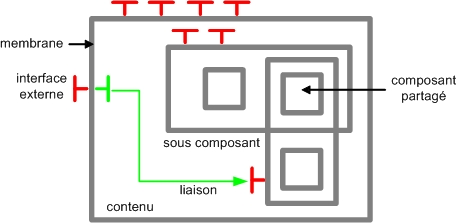
\includegraphics{img/fractal_component}
%   \caption{Exemple d'un modèle \fractal{} de composants} %la légende
%  \label{fig:Comp} %la légende
% \end{figure}


 %on ferme l'environnement figure
% Pour avoir un interligne de 1,5
% \input{P0}
%\input{P01}
% \input{P1}
% \input{P2}
% \input{annexereal}

% Pour finir l'interligne de 1,5

\printindex

\appendix
\bibliographystyle{alpha}
\bibliography{biblio.bib}

\end{document}
